\section{Grammatical approach}

Trees of triples can be produced after analysing the grammatical structure of sentences.
We developed a module in Python which produces triples using this grammatical approach\footnote{\url{https://github.com/ProjetPP/PPP-NLP-classical/}}.
First, we  present the tool we use to extract grammatical dependencies. Then, we expose chronologically our algorithm to product triples from grammatical structure.

We will detail throughout this section our algorithm on the example:
\begin{center}
 \textit{What is the birth date of the president of the United States?}
\end{center}

%########################################################################################%

\subsection{\Stanford}

The \Stanford library \footnote{\url{http://nlp.stanford.edu/software/corenlp.shtml}} is a tool developed by the \emph{Stanford Natural Language Processing group}, composed of linguists and computer scientists. This software is well-documented and considered as a ``state of the art'' tool. Moreover, it includes very efficient grammatical parsers.

Since this library is written in Java, and our module in Python, we use a Python wrapper\footnote{\url{https://bitbucket.org/ProgVal/corenlp-python/overview}} we first patched to support Python 3 and some features the wrapper did not implement.

We use \CoreNLP mostly to get grammatical dependency trees from input questions. It consists in trees which nodes are the words of the sentence, and edges reflect the grammatical relations between words.

Figure \ref{tree_one} provides an overview of such a tree on our question example \emph{What is the birth date of the president of the United States?}. For instance, the edge:
  \[\texttt{president}\xrightarrow{\texttt{det}}\texttt{the}\]
means that \emph{the} is a determiner for \emph{president}.

\begin{figure}
  \centering
  \caption{Dependency tree}
  \label{tree_one}
    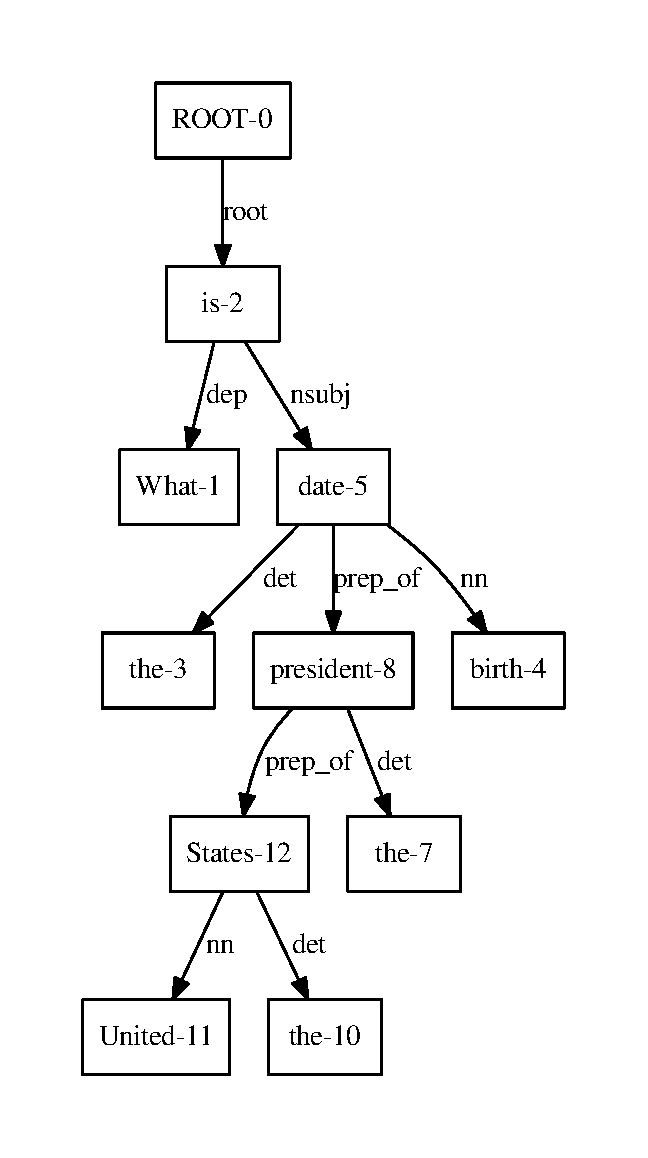
\includegraphics[scale=0.6]{../examples_NLP_grammatical/tree1.pdf}
\end{figure}

Some nodes of this tree are also endowed with tags. For example, \emph{United} and \emph{States} have the tag \emph{location}.

The Stanford typed dependencies manual (\cite{stanfordDep}) provides a full list and description of possible grammatical dependencies.

%########################################################################################%

\subsection{Preprocessing}

The preprocessing consists in a sequence of operations executed on the tree output by the \Stanford library. The aim is to simplify it, by merging the nodes which should belong together. % Do not put an 's' at the end of 'output', it is in past participle form. Moreover, 'output' seems to be preferred to 'outputted': http://english.stackexchange.com/questions/35418/past-tense-of-to-output-output-or-outputted

The current version of the module performs two sorts of merges:
\begin{itemize}
    \item \textbf{Merge quotation nodes.} This operation merges all the nodes which are in a same quotation (delimited by quotation marks). It also adds the words
    of the quotation which were deleted by the \Stanford library (e.g. \emph{in}, \emph{of}\dots). The final result is a node, containing the
    exact quotation, and placed at the appropriate position in the tree.
    
    \item \textbf{Merge named entities.} The \Stanford library performs a \emph{named entities recognition} (NER), which provides informative 
    tags for some nodes. For instance, \emph{United} and \emph{States} are tagged \emph{LOCATION} (see figure \ref{tree_two}). In the preprocessing step, we merge all neighbour nodes with a same NER tag. In our example, we merge the two nodes \emph{United States} into one single node.
\end{itemize}

The preprocessing also identifies the question word (Who, What, Where\dots) and removes it from the dependency tree.

Preprocessing is illustrated on figure \ref{tree_two}. The question word is \textit{What}.

\begin{figure}
  \centering
  \caption{Dependency tree preprocessed}
  \label{tree_two}
    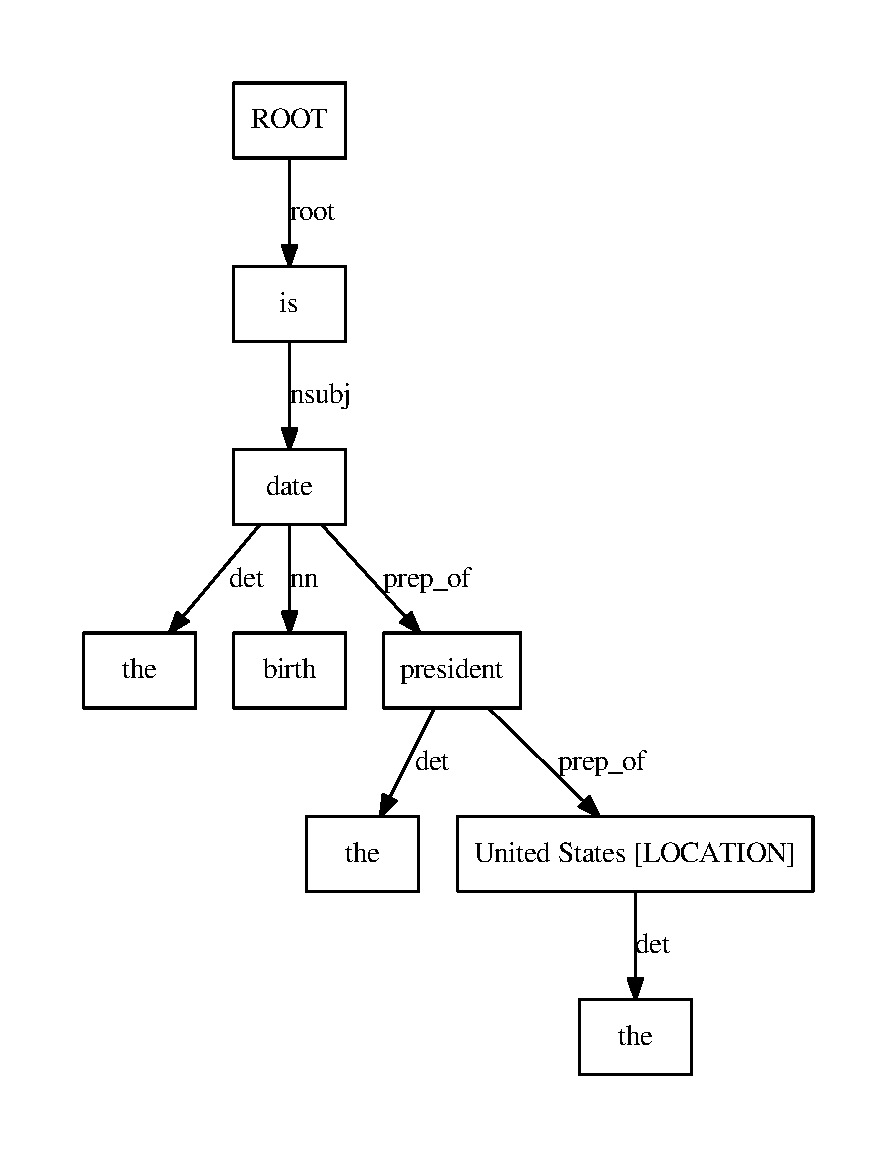
\includegraphics[scale=0.6]{../examples_NLP_grammatical/tree2.pdf}
\end{figure}

%########################################################################################%

\subsection{Grammatical dependencies analysis}

The grammatical tree is simplified by applying one of the following rules to each edge:
\begin{itemize}
 \item remove the edge and its endpoint node. For instance, a \textit{dep} relation, such as \textit{the} in our example, is often removed.
 \item merge the two nodes of the edge. Merge operations try to gather words of a same expression (e.g. phrasal verbs) that have not been merged during preprocessing.
 \item tag the edge with a ``triple production rule''.
\end{itemize}

The third operation is the most important. Dependencies relations are replaced by a restricted set of tags that will enable us to product a triples tree thereafter.

On our example, the edge:
\[\texttt{birth}\xrightarrow{\texttt{nn}}\texttt{date}\]

is merged into a single node : \textit{birth date}.

One of the triples production rules tag is : 

\[\texttt{is}\xrightarrow{\texttt{t1}}\texttt{birth date}\]

The simplified tree of our example is illustrated on figure \ref{tree_three}.

\begin{figure}
  \centering
  \caption{Dependency tree simplified}
  \label{tree_three}
    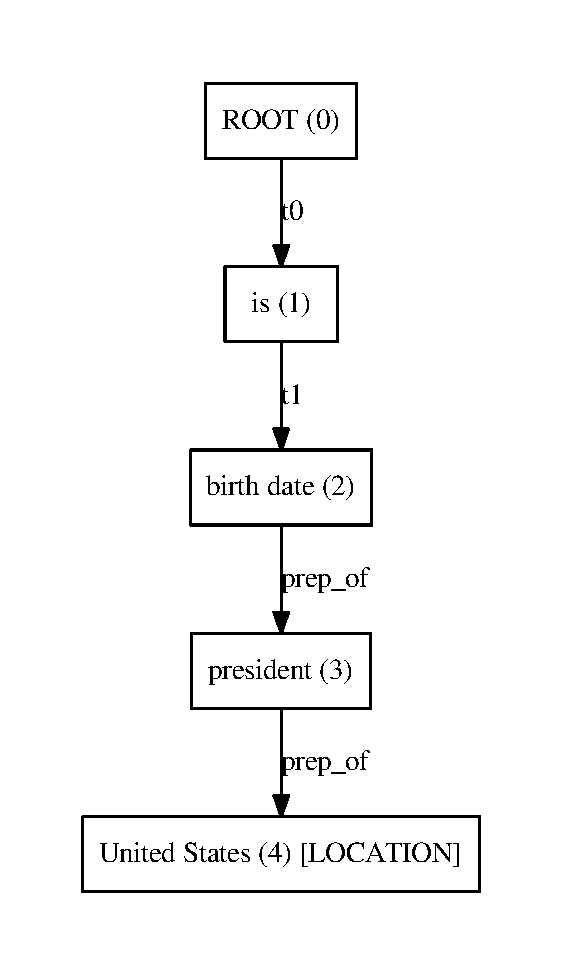
\includegraphics[scale=0.6]{../examples_NLP_grammatical/tree3.pdf}
\end{figure}

%########################################################################################%

\subsection{Triples production}

The triples production is the final step. It outputs the triples tree.

First, we assign a number to each remaining node. The root of the tree has always number \textit{0}. We have directly printed these numbers on figure \ref{tree_three}.

Then, we associate to each subtree of root's number \textit{x} an unknown denoted \textit{?x} that identifies the information the subtree refers to. On our example, the subtree of root \textit{president} (number \textit{3}) represents the name of the president of the United States. This unknown is denoted \textit{?3}.

Unknowns are linked together into triples thanks to the triples production rules tagged previously. For instance, an  edge tagged \textbf{t2}:

\[\texttt{a}\xrightarrow{\texttt{t2}}\texttt{b}\]

products the triples \hl{(?a,a,?b)}, or \hl{(?a,a,b)} if b is a leaf (a and b are replaced by the words of the node they refer to).

The tag \textbf{t1} directly links two unknowns \hl{?a = ?b}, instead of producing a triple.

The tag \textbf{t0} products nothing.

We obtain the following result on our example:

\begin{center}
 ?1 = ?2 ~\\
 (?2 , birth date of , ?3) ~\\
 (?3 , president of , United States)
\end{center}

Then, we link \textit{?0} to \textit{?1}, depending on the question word of the question. Here we have (question word \textit{What}):
\begin{center}
 (?1,definition,?0)
\end{center}

The four previous rules are simplified into a set of triples:

\begin{center}
 (?1,definition,?0) ~\\
 (?1 , birth date of , ?3) ~\\
 (?3 , president of , United States)
\end{center}

Find an answer to the question is equivalent to build a model of the conjunctive formula: \textbf{(?1 , definition , ?0)$\wedge$(?1 , birth date of , ?3)$\wedge$(?3 , president of , United States)} and outputs the value of \textit{?0}.

The triples tree is obtained by replacing each unknown \textit{?x} by a triple containing \textit{?x} \textit{and not} \textit{?0}. The final result, taken from the PPP website, is printed on figure \ref{tree_four}. Figure \ref{triple_tree} contains the formal representation of the triples tree of our example.

\begin{figure}[!h]
  \centering
  \caption{Triples tree}
  \label{tree_four}
    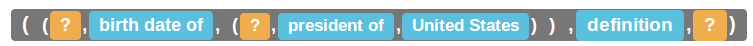
\includegraphics[scale=0.5]{../examples_NLP_grammatical/final_result.png}
\end{figure}

Backend modules (such as Wikidata module) will have to fill intermediate unknowns : \hl{((August 4 1961,birth date of, (Barack Obama, president of, United States)), definition, ?)} and finally provide the final answer that replaced \textit{?} (for example: a description of the August 4 1961 date).


%########################################################################################%

\subsection{Future work}

\subsubsection{Grammatical rules analysis}

Our analysis of grammatical rules, in order to product triples, is very basic. Currently, we only have about 5 rules. Although it is good enough to handle a lot of questions, we are not able to process conjunctions for example (e.g. \textit{``Who wrote "Lucy in the Sky with Diamonds" and "Let It Be"?''}).

\subsubsection{Preprocessing merging}

There remains nodes which should stay together but are not merged by our module, for instance \emph{prime minister} or \emph{state of the art}. Recognizing such words is called \emph{Multiword Expressions Processing}. This task is a whole part of Natural Language Processing theory. 

We have several tracks to improve merging. Existing algorithms or softwares need to be tested. We could also use multiword expressions dictionaries.

\subsubsection{Question type analysis}

The current algorithm attaches great importance to the type of the input question. Sentences starting by a question word (Who, Where, How\dots) are better processed than Yes/No questions for instance.

\subsubsection{Triples tree improvement}

The triples tree will be improved to take into account new types of nodes, adapted to databases queries. For example, a node could be tagged ``FIRST'' to pick the first occurrence of a list of answers (e.g. \hl{FIRST(?,presidents of, United States)}).
